\subsubsection{\stid{1.14} GASNet-EX}\label{subsubsect:gasnet-ex}
\paragraph{Overview} 

The Lightweight Communication and Global Address Space Support project (Pagoda)
is developing GASNet-EX~\cite{gasnet-site}, a portable high-performance communication layer
supporting multiple implementations of the Partitioned Global Address Space
(PGAS) model.
GASNet-EX clients include Pagoda's PGAS programming interface UPC++~\cite{Bachan:paw17,upcxx-site}
 and the Legion Programming
System~\cite{bauer2012legion,legion-site} (WBS~2.3.1.08).

GASNet-EX's low-overhead communication mechanisms are designed to maximize
injection rate and network utilization, tolerate latency through
overlap, streamline unpredictable communication events, minimize
synchronization, and efficiently support small- to medium-sized
messages arising in ECP applications.  GASNet-EX enables the ECP
software stack to exploit the best-available communication mechanisms,
including novel features still under development by vendors.  The
GASNet-EX communications library and the PGAS models built upon it
offer a complementary, yet interoperable, approach to MPI with OpenMP,
enabling developers to focus their effort on optimizing
performance-critical communication.

We are co-designing GASNet-EX with the UPC++ development team with
additional input from the Legion and
(non-ECP) Cray Chapel~\cite{chapel-chapter,chapel-site} projects.

\paragraph{Key  Challenges}

Exascale systems will deliver exponential growth in on-chip parallelism and
reduced memory capacity per core, 
increasing the importance of strong
scaling and finer-grained communication events.  
Success at Exascale demands that
software needs to minimize the work performed by lightweight cores and avoid the
overhead of long, branchy serial code paths; 
this motivates a requirement for efficient
fine-grained communication.
These problems are exacerbated by application trends; many of the ECP applications require
adaptive meshes, sparse matrices,
or dynamic load balancing.
All of these characteristics favor the use of
low-overhead communication mechanisms that
can maximize injection rate and network utilization, tolerate latency through
overlap, accommodate unpredictable communication events, minimize synchronization,
and efficiently support small- to medium-sized messages. The ECP software stack
needs to expose the best-available communication mechanisms, including novel
features being developed by the vendor community.

\paragraph{Solution Strategy}

The PGAS model is a powerful means of addressing these
challenges and is critical in building other ECP programming systems,
libraries, and applications.  We use the term {\em PGAS} for models that support
one-sided communication, 
including contiguous and non-contiguous remote memory access (RMA) operations such as put/get
and atomic updates. Some of these models also include support for remote function invocation.
GASNet-EX~\cite{gasnet-lcpc18} is a communications library that provides the foundation for implementing
PGAS models, and is the successor to the widely-deployed GASNet library.
We are building on over 15 years of experience with the GASNet~\cite{gasnet-spec,gasnet-site}
communication layer to provide production-quality implementations that include
improvements motivated by
technology trends and application experience.  

The goal of the GASNet-EX work is to provide a portable, high-performance GAS
communication layer for Exascale and pre-Exascale systems, addressing the challenges
identified above.
GASNet-EX provides interfaces that efficiently match the RDMA capabilities of modern
inter-node network hardware and intra-node communication between distinct address spaces.
New interfaces for atomics and collectives have enabled offload to current
and future network hardware with corresponding capabilities.
These design choices and their implementations supply the low-overhead communications
mechanisms required to address the requirements of Exascale applications.

\begin{figure}[htb]
  \centering
  \subfloat[8-byte RMA Latencies\label{fig:rma-lat-bars}]{
     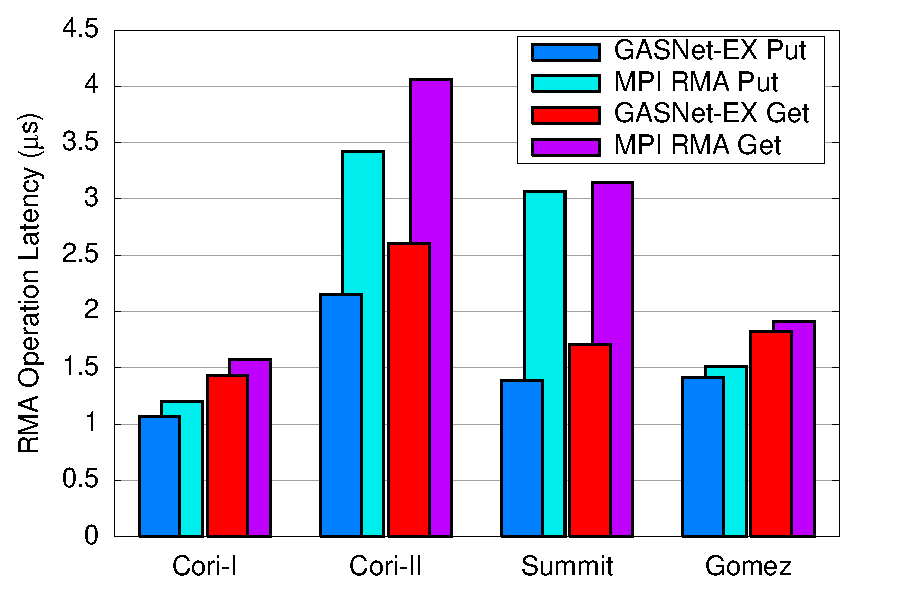
\includegraphics[width=0.432\textwidth]{projects/2.3.1-PMR/2.3.1.14-UPCxx-GASNet/latency_bars.pdf}
  }
  \subfloat[Summit Flood Bandwidth\label{fig:summit-bw}]{
     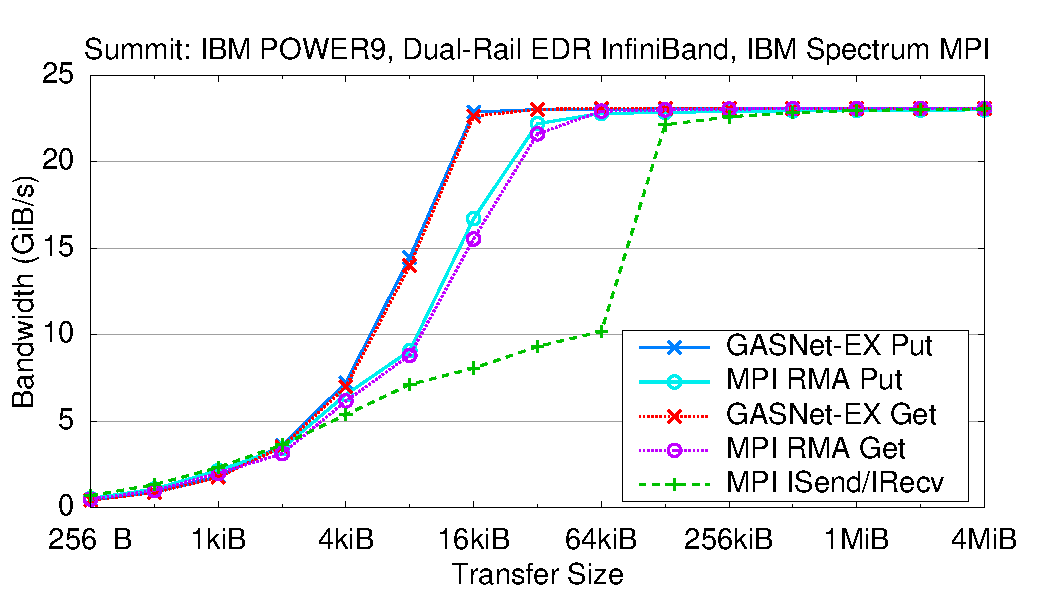
\includegraphics[width=0.504\textwidth]{projects/2.3.1-PMR/2.3.1.14-UPCxx-GASNet/Summit-slide-BW.pdf}
  }
  \caption{\label{fig:gasnet-ex-rma} Selected GASNet-EX vs. MPI RMA Performance Results}
\end{figure}

Figure~\ref{fig:gasnet-ex-rma} shows representative results from a
paper~\cite{gasnet-lcpc18} comparing
the RMA performance of GASNet-EX with MPI on multiple systems including
NERSC's Cori and OLCF's Summit%
\footnote{The paper's results from Summitdev
have been replaced by more recent (June 2019) results from OLCF's newer Summit system.}.
These results demonstrate the ability of a PGAS-centric runtime to
deliver performance as good as MPI, and often better.
%
The paper presents experimental methodology and system descriptions, which are
also available online~\cite{gasnet-site}, along with results for additional
systems.

Figure~\ref{fig:rma-lat-bars} shows the latency of 8-byte RMA Put and Get operations on
four systems, including two distinct networks and three distinct MPI
implementations.
%
GASNet-EX's latency is 6\% to 55\% better than MPI's on Put and 5\% to 45\%
better on Get.
%
Algorithms sensitive to small-transfer latency may become practical in PGAS
programming models due to these improvements relative to MPI.

Figure~\ref{fig:summit-bw} shows flood bandwidth of RMA Put and Get over the
dual-rail InfiniBand network of OLCF's Summit.
GASNet-EX's bandwidth is seen to rise to saturation at smaller
transfer sizes than IBM Spectrum MPI, with the most pronounced differences
appearing between 4KiB and 32KiB.
%
Comparison to the bandwidth of MPI message-passing (dashed green series) illustrates the
benefits of one-sided communication, a major feature of PGAS models.


\paragraph{Recent Progress}

Work on GASNet-EX in the past year has covered several distinct areas.

Co-design work is on-going with the UPC++, Legion and Chapel developers.  These
interactions are bi-directional, guiding design and implementation decisions
made in GASNet-EX as well as in the client runtimes.
%
Recent work~\cite{gasnet-reassembly} for the Cray Aries network has yielded
significant performance improvement on systems of importance to UPC++ and Legion.
Specifically, implementation of a new target-side reassembly protocol improved
AM Long end-to-end latency by up to 33\%, and the effective bandwidth by up to
49\%, while also enabling asynchronous source completion that drastically reduces
injection overheads.

We have begun work to improve interoperability of GASNet-EX and MPI within the
same executable.  Together with the Exascale MPI project (WBS~2.3.1.07) we have
developed an initial implementation of a small library to manage cooperative
progress of multiple communications runtimes.  We have demonstrated the ability
of this library, with suitable calls added to GASNet-EX and MPICH, to resolve
two canonical examples of the class of deadlock it is meant to prevent.

We have completed work to leverage features of the InfiniBand network
present in OLCF's Summit.  One such development is modifications to fully
utilize the multiple InfiniBand network ports (a.k.a ``rails'') in a Summit
node.  Another is use of Mellanox's ``ODP'' (On-Demand Paging) to provide
efficient and robust RDMA transfers to and from memory in a processes' stack
and dynamic heap.

\paragraph{Next Steps}

Our next efforts include:
\begin{enumerate}

\item \textbf{Device (GPU) Memory Support}.
GASNet-EX's RMA APIs have been designed to enable hardware offload of
transfers to and from GPU memories (\textit{e.g.} use of GPUDirect).
Near-future work includes implementation of this capability for OLCF's
Summit.  This work includes adding support for multiple
communications endpoints and multiple memory segments, which also provide
benefit to multi-threaded runtimes by reducing contention for shared resources.

\item \textbf{Specialization for InfiniBand}.  Network-specific implementations
of new GASNet-EX features for the InfiniBand network will provide performance
benefits on systems such as OLCF's Summit.  The benefits of such specialization
for the Cray Aries network has been demonstrated previously~\cite{gasnet-aries}.

\item \textbf{Client-Driven Tuning}.  In collaboration with authors of client
runtimes using GASNet-EX (most notably UPC++ and Legion) and their users (such
as ExaBiome), we will continue to identify and address any significant
bottlenecks or performance anomalies which are discovered.

\end{enumerate}
